\section{Principles of tile algorithms}\label{sec:tile}
In order to use modern many/multi-core shared memory architectures at
full efficiency,
many LAPACK library algorithms initially powered by
block algorithms have been redesigned into tile algorithms.
This led to a new generation of linear algebra libraries such as
PLASMA~\cite{DBLP:journals/corr/abs-0709-1272}.
The key idea is that,
instead of operating on block-columns as found in LAPACK,
tile algorithms operate at a finer granularity by dividing the whole
matrix into small square tiles which are more likely to fit into the
L2 cache of a CPU.
As illustrated in Figure~\ref{fig:SVD_initial}, the original
matrix has been converted into a 5-by-5 tile matrix.  One of the
advantages of working at the tile level is that it provides more
room for parallelism with many tasks to keep all computational cores
busy.

Another advantage of tile algorithms is that they alleviate
the fork-join overhead inherent to parallelized LAPACK
block algorithms~\cite{haidar2012analysis}.
In fact,
the order of execution of the tasks in tile algorithms are commonly
represented in form of a Directed Acyclic Graph (DAG) where each node
represents a task, while the edges represent the
data dependencies between the tasks.
These tasks are then scheduled
by a runtime system which checks the dependencies and
takes care of launching tasks on appropriate cores.

  \begin{figure}[h!]
    %%%% 1
    \captionsetup[subfigure]{justification=justified,singlelinecheck=false}
  \begin{subfigure}[t]{0.160 \textwidth}
    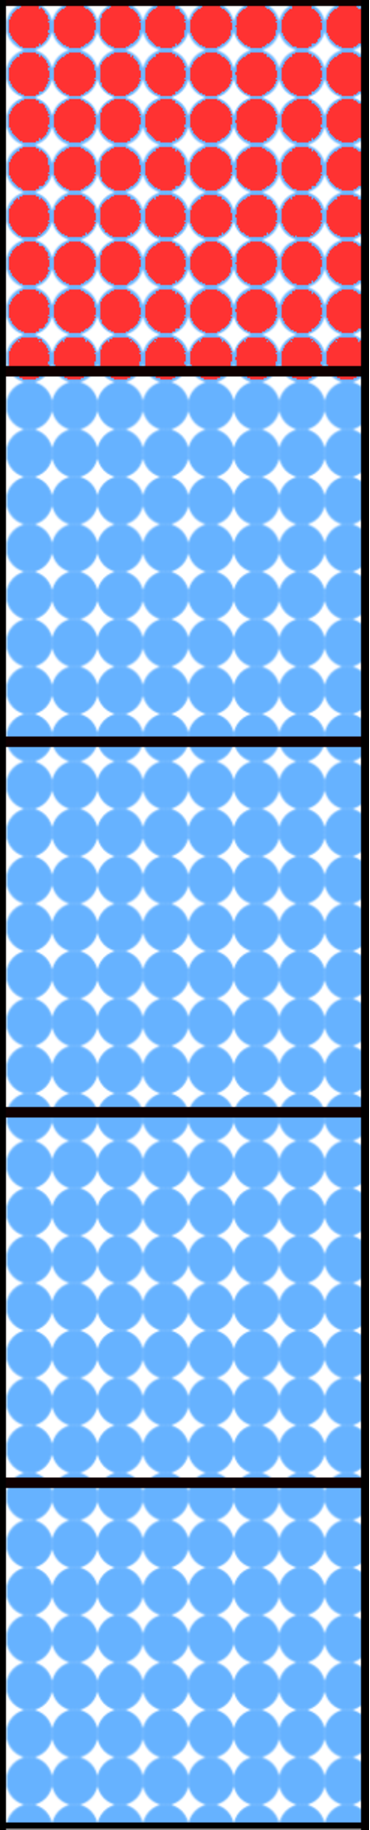
\includegraphics[width=0.7cm, height=3.5cm]{fig/SVD_rect_panel_1}
    \caption{\label{fig:geqrt_1}QR}
  \end{subfigure}
  \hfill
  %%%% 2
  \begin{subfigure}[t]{0.160 \textwidth}
    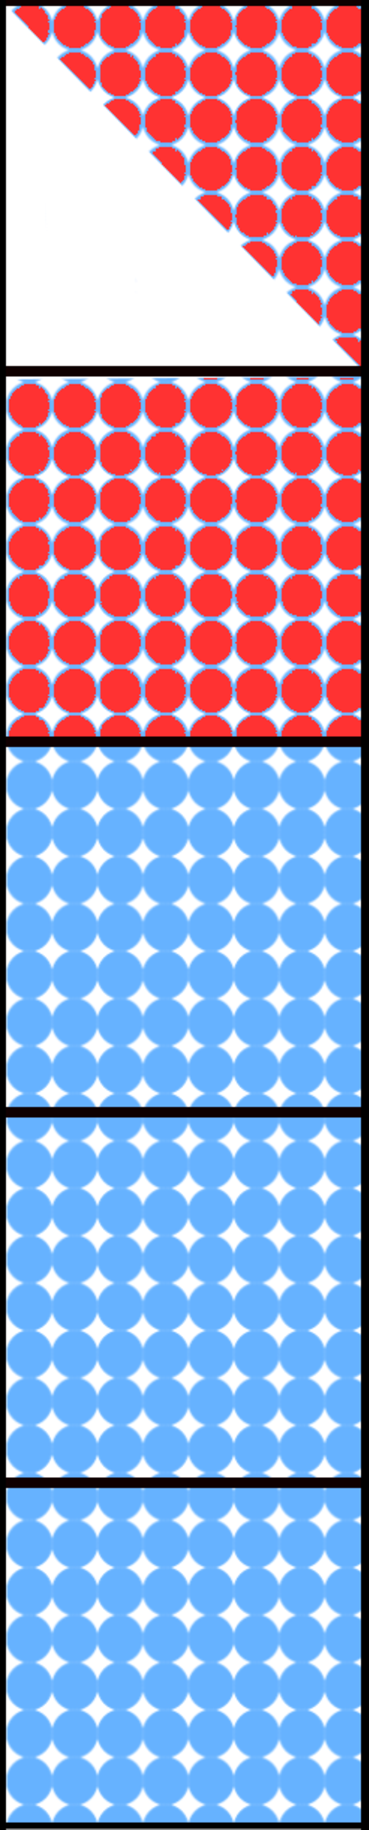
\includegraphics[width=0.7cm, height=3.5cm]{fig/SVD_rect_panel_3}
    \caption{\label{fig:tsqrt_2}TSQRT}
  \end{subfigure}
  \hfill
  %%%% 3
    \begin{subfigure}[t]{0.160 \textwidth}
    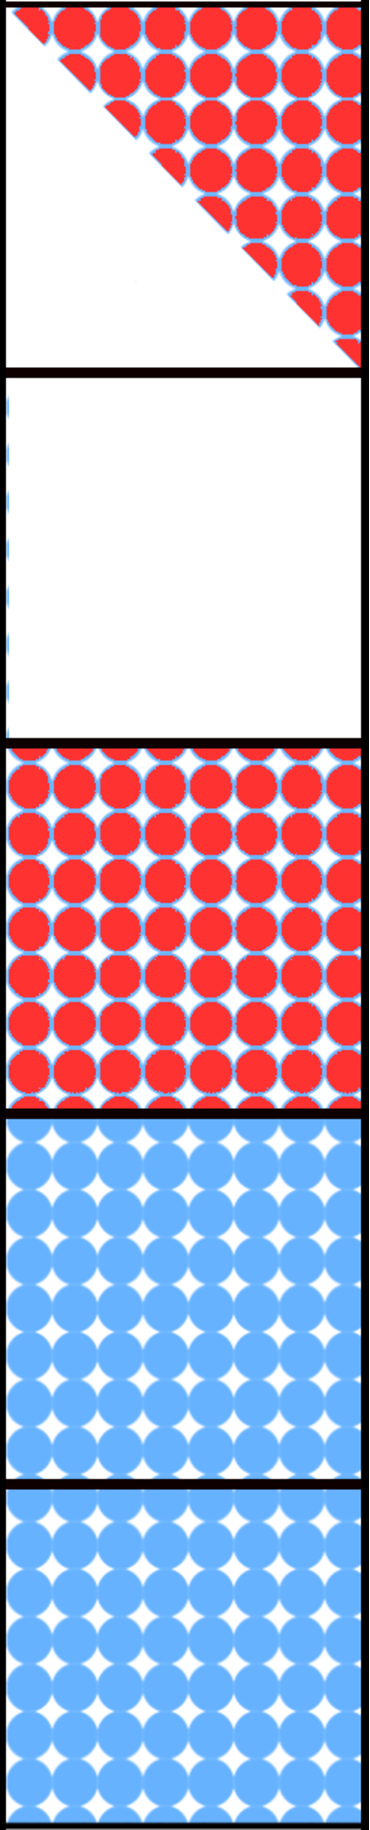
\includegraphics[width=0.7cm, height=3.5cm]{fig/SVD_rect_panel_5}
    \caption{\label{fig:tsqrt_3} TSQRT}
    \end{subfigure}
    \hfill
    %%%% 4
    \begin{subfigure}[t]{0.160 \textwidth}
      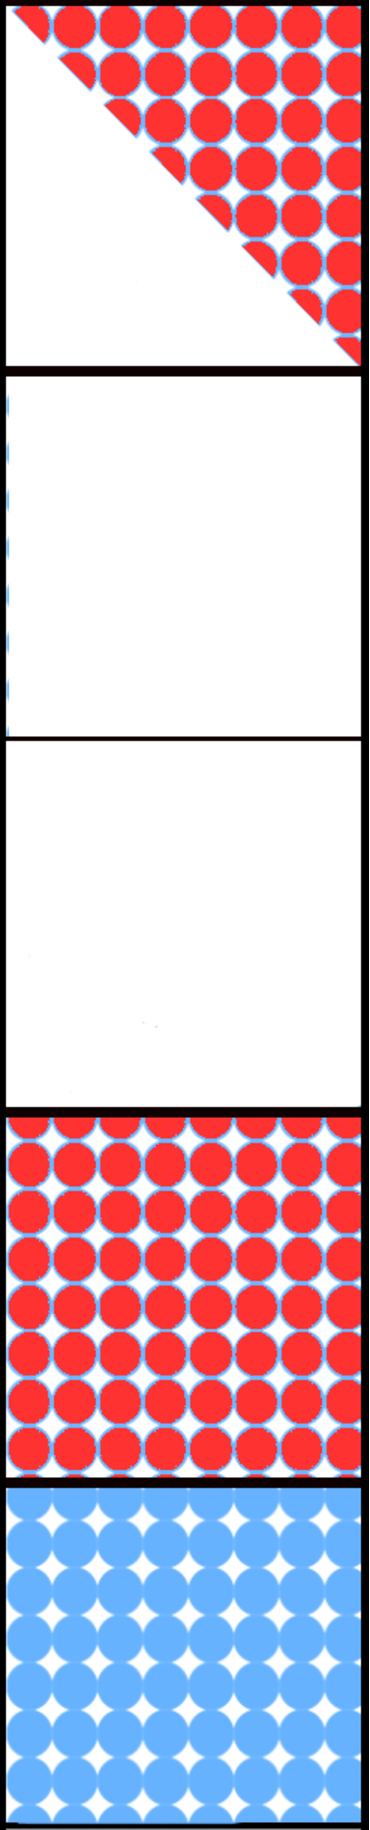
\includegraphics[width=0.7cm, height=3.5cm]{fig/SVD_rect_panel_6}
      \caption{\label{fig:tsqrt_4}TSQRT}
    \end{subfigure}
    \hfill
    %%%% 5
    \begin{subfigure}[t]{0.160 \textwidth}
      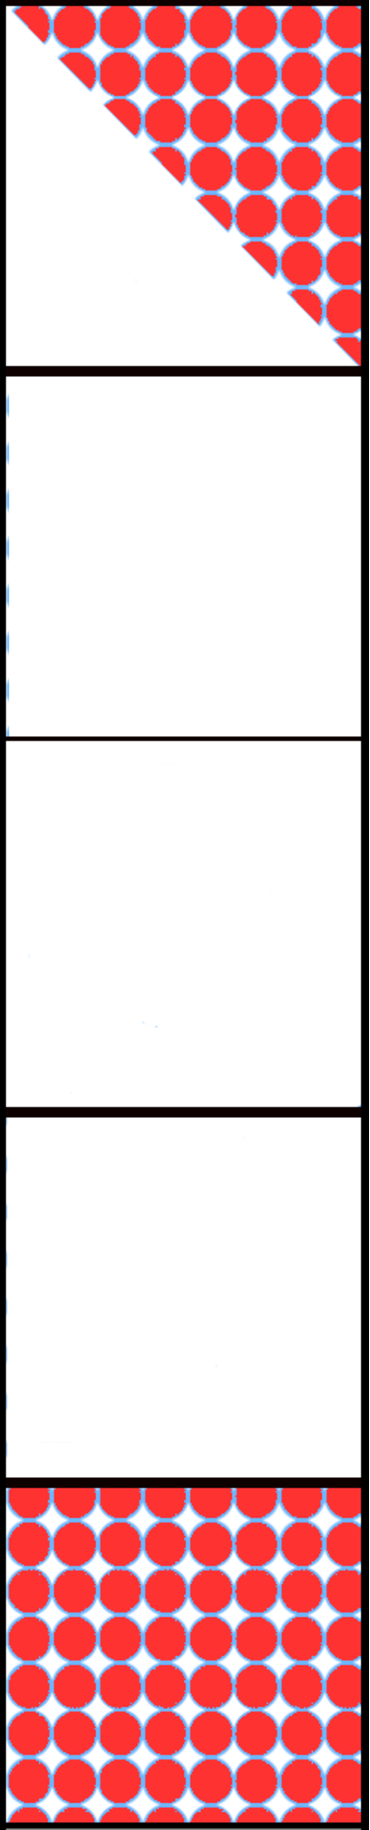
\includegraphics[width=0.7cm, height=3.5cm]{fig/SVD_rect_panel_7}
      \caption{\label{fig:tsqrt_5}TSQRT}
    \end{subfigure}
    \hfill
    %%%% 6
    \begin{subfigure}[t]{0.160 \textwidth}
      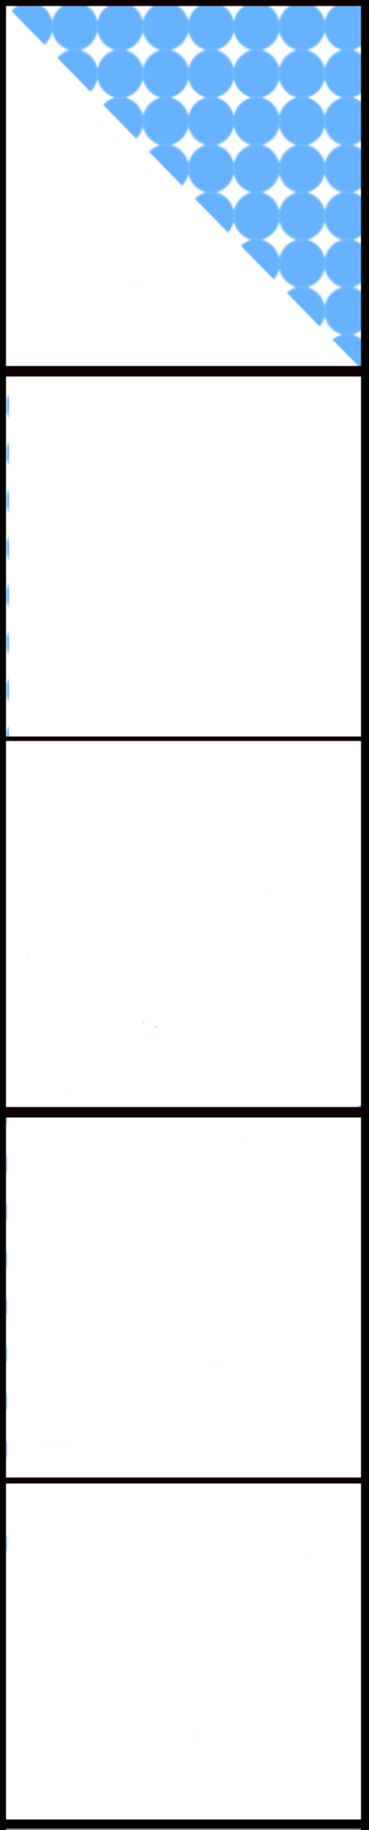
\includegraphics[width=0.7cm, height=3.5cm]{fig/SVD_rect_panel_8}
      \caption{\label{fig:tsqrt_output}End}
    \end{subfigure}
    \caption{Panel factorization using the triangle on top of square QR factorization kernel (TSQRT).
    \label{fig:rect_panel}}
\end{figure}

For the sake of illustration, Figure~\ref{fig:rect_panel}
shows the tile algorithm variant of QR factorization for a panel
(block-column).
Following the example shown in Figure~\ref{fig:two_stage},
the panel has been divided into 5 tiles.
This algorithm involves two tile kernels:
a standard QR factorization kernel to
factorize the top-most tile (Figure~\ref{fig:geqrt_1}),
and a specialized kernel to use the top triangular matrix
from the first QR factorization
to eliminate the square tiles below
(Figures~\ref{fig:tsqrt_2}-\ref{fig:tsqrt_5}).
This kernel is denoted TSQRT and stands
for ``triangle on top of square tile QR factorization''.
In the next few sections we will introduce other specialized kernels
that we designed  to operate on tiles.
